\section{Protocolos de autenticação}
\label{auth_protocols}
\quad Neste caso os protocolos servem para verificar com o provedor de identidade se um utilizador inseriu a senha certa de uma conta na interface da \textit{helper application}.

\subsection{Protocolo iterativo de autenticação usando técnicas de conhecimento nulo}

\quad Umas das componentes principais deste projeto é a autenticação usando o protocolo ZKP, que permite realizar processos de autenticação (pela prova de conhecimento de um segredo partilhado) sem que o próprio segredo tenha que percorrer um determinado canal de comunicação. Neste caso o processo de autenticação é realizado entre uma aplicação auxiliar, que é executada localmente no dispositivo do utilizador, e um IDP. Conceptualmente o IDP armazena dados de autenticação de um determinado utilizador \textit{(username, email, password, etc)}, e para que o processo de autenticação seja efetuado com sucesso pelo utilizador, é necessário este provar ao IDP que sabe a senha associada a uma determinada conta (que vai ser o segredo partilhado), esta prova de conhecimento é realizada através de um protocolo de comunicação entre a aplicação auxiliar do utilizador e o provedor de identidade, que vai ser explicado nesta secção.

\subsubsection{Carateristicas protocolares do ZKP}

\begin{itemize}
    \item Este protocolo vai ter uma natureza iterativa, isto é, ambas as entidades vão trocar mensagens até estas terem a convicção suficiente que a outra entidade tem conhecimento do segredo partilhado.
    \item Devido à caraterística anterior é necessário definir um numero de iterações mínimas, digamos \textbf{N}, que vai representar o número de mensagens enviadas por cada entidade durante a execução deste protocolo. Portanto, no final, este processo vai ter pelo menos \textbf{2N} mensagens trocadas. Na fase de definição do protocolo ZKP, deve ser assumido que ambas as entidades contribuem para a definição do valor de \textbf{N}. Em principio, quanto maior for o \textbf{N}, mais seguro é o protocolo mas também consome mais recursos computacionais e de rede, portanto é essencial encontrar uma solução equilibrada que faça o balanceamento entre a qualidade da autenticação e a prevenção de negação de serviço.
    \item Cada mensagem trocada neste protocolo deve ter os seguintes parâmetros:
    \begin{itemize}
        \item \textbf{challenge}, que representa o valor de um desafio aleatório
        \item \textbf{r}, que é um representa um \textit{bit} (0-1), que vai ser o parâmetro usado para verificar o estado do protocolo
    \end{itemize}
    \item O valor de \textbf{r} deve ser calculado tendo em conta todos os desafios recebidos e enviados até à iteração \textbf{i} e a senha partilhada \textbf{P}. \footnote{Todos os detalhes matemáticos serão clarificados na secção \ref{mat_zkp}}
    \item Se em algum momento o valor de \textbf{r} recebido estiver incorreto, o recetor saberá imediatamente que o outro participante não é legitimo, mas ainda assim vai continuar a execução do protocolo com a pequena diferença que os valores de  \textit{r} vão ser números totalmente aleatórios. Desta forma, a entidade maliciosa não vai receber valores genuínos após a resposta errada, evitando que este obtenha dados suficientes para executar um ataque de adivinhação com sucesso.
\end{itemize}

\subsubsection{Considerações gerais na implementação do protocolo ZKP}

\quad Uma vez que este protocolo de autenticação vai ser executado num ambiente \textit{Web}, onde existe a clara estrutura de um modelo cliente-servidor, o intercâmbio de mensagens entre as entidades vai ser realizado seguindo o mesmo modelo. Neste caso o IDP vai ter o papel de servidor e a aplicação auxiliar o papel de cliente, isto é, todo o fluxo de execução deste protocolo vai ser iniciado pela aplicação auxiliar. Esta caraterística além de se enquadrar deveras bem no contexto de protocolos \textit{Web}, também acaba por agilizar os trabalhos de implementação uma vez que (teoricamente) o IDP é uma entidade pública que está associada a um domínio público e é acessível do exterior (internet), e portanto, deverá ser trivial enviar um pedido para o IDP. 

\subsubsection{Algoritmo para escolha de N e cálculo de r no protocolo ZKP}
\label{mat_zkp}

\quad Uma das capacidades deste protocolo é o facto de ser iterativo e portanto é necessário definir um número mínimo de iterações \textbf{N}. Durante a implementação do algoritmo de negociação do número de iterações (que em termos de implementação corresponde ao número de mensagens enviadas por cada entidade), o valor de \textbf{N} passa a representar exatamente o número de iterações do protocolo. O algoritmo consiste na partilha mútua de um intervalo que representa o número mínimo e máximo de iterações aceitáveis por cada entidade, onde o servidor verifica se existe uma intersecção válida entre esses dois conjuntos, e caso exista, o maior valor (do conjunto proveniente da intersecção) é escolhido e, posteriormente, enviado para a \textit{helper application} - \ref{lst:alg_N}.

\begin{minipage}{\linewidth}
    \begin{lstlisting}[language=C, caption={Algoritmo de escolha do valor de N.}, label={lst:alg_N}, escapeinside={(*}{*)}]
        helper_application_n_interval = (50, 300)
        idp_n_interval = (200, 1000)
        intersection = (*$helper\_application\_n\_interval \cap idp\_n\_interval$*)
        chosen_N = max(intersection) // Send this value to the helper application
    \end{lstlisting}
\end{minipage}

\quad Para cumprir com a caraterística principal deste protocolo (o facto de ser um protocolo iterativo) é necessário implementar um protocolo de \textbf{desafio-resposta} entre as duas entidades participantes, e durante a execução do protocolo o segredo partilhado não deve navegar no canal de comunicação. Portanto, como explicado anteriormente as duas entidades irão trocar mensagens cujo conteúdo deve conter um desafio aleatório \textbf{C} e um bit \textbf{r} que deve ser calculado tendo em conta todos os desafios trocados e a senha partilhada \textbf{P}.

\quad Considerando que \textbf{$R_i$} representa a resposta calculada a partir de todos os desafios trocados até à iteração \textbf{i}, \textbf{r} vai ser o valor de paridade \footnote{A paridade de um número refere-se ao facto de conter um número ímpar ou par de bits a 1. Neste caso os valores vão ser 0 caso seja par e 1 caso seja ímpar} de \textbf{$R_i$} . Portanto é necessário implementar um algoritmo capaz de calcular os valores de \textbf{R} tendo em conta a senha partilhada e os desafios enviados -  \ref{lst:alg_F_RI}.


\begin{minipage}{\linewidth}
    \begin{lstlisting}[language=C, caption={Algoritmo usado para calcular o valor de r.}, label={lst:alg_F_RI}, escapeinside={(*}{*)}]
        def f(challenge, password, previous_response=None):
            if previous_challenge is not None:
                password = HMAC(password, previous_response)
            
            return HMAC(password, challenge) // HMAC(key, message)

        (*$R_i = f(C_i, P, R_{i-1})$*)
        (*$r_i = parity(R_i)$*)
        
    \end{lstlisting}
\end{minipage}

\quad Para permitir a implementação deste processo algorítmico, foi usada uma função de \textit{hash} criptográfica que tem como objetivo providenciar autenticação de mensagens usando um segredo partilhado - \textbf{HMAC} \cite{hmac}. O \textit{HMAC} recebe como argumentos de entrada um segredo partilhado e uma mensagem para ser autenticada (para garantir que esta não foi adulterada) e retorna um \textit{blob} binário irreversível (isto é, não é possível transformar os dados de saida nos argumentos de entrada) e completamente diferente da mensagem de entrada \footnote{Obviamente que este valor pode ser usado pela entidade recetora para verificar a integridade da mensagem, mas para este caso especifico não vai ser usado esta propriedade}. No contexto deste problema, o segredo partilhado vai ser a senha do utilizador e a mensagem será o desafio gerado aleatoriamente, a escolha desta função é justificada pelo facto de permitir gerar transformações matemáticas irreversíveis sobre duas instâncias de dados (a senha e o desafio aleatório), o que permite às duas entidades calcular o mesma resposta caso a senha e o desafio seja iguais. Contudo, o simples uso da função HMAC não chega para cumprir os requisitos do calculo do valor de \textbf{R} uma vez que este tem de ser calculado tendo em conta todos os desafios trocados até uma determinada iteração e neste momento só é possível calcular \textbf{R} tendo em conta apenas um desafio, por isso, para cumprir esta caraterística antes de executar a função de \textit{hash} criptográfica sobre o desafio recém calculado, é calculado o \textit{HMAC} sobre a resposta calculada na iteração anterior que depois é passado com segredo na segunda execução do HMAC sobre o desafio. Com este encadeamento de operações os \textbf{R} irão ser calculados tendo em conta o valor de todos os desafios, mas de uma forma implícita e indireta. Por fim, basta apenas calcular \textbf{r} que é o valor de paridade da resposta recém calculada. Para finalizar apenas de referir que não é usada a senha em \textit{clear text} como segredo partilhado, mas sim o \textit{digest} da senha usando a função de \textit{hash} \textbf{SHA-512}.

\quad Para esclarecer, caso umas das entidades envie o valor errado de \textbf{r} numa das mensagens, a entidade recetora irá calcular o valor de \textbf{r} aleatoriamente não procedendo mais ao cálculo do valor da paridade de \textbf{R}, e portanto, o protocolo irá executar as iterações combinadas inicialmente mas com valores completamente errados o que provocará uma falha no processo de autenticação.


\subsubsection{Fluxo de execução do protocolo}

\begin{figure}[H]
    \caption{Protocolo ZKP}
    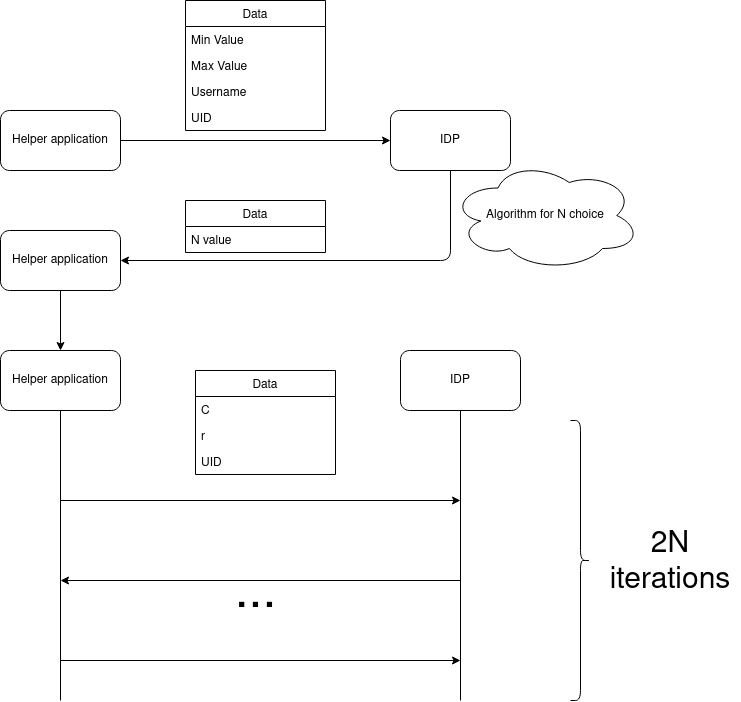
\includegraphics[width=\textwidth]{img/zkp.png}
    \centering
\end{figure}


\quad Como já foi referido anteriormente, a aplicação auxiliar inicia o processo de autenticação usando o protocolo de conhecimento nulo, portanto temos:
\begin{enumerate}
    \item A \textit{helper application} envia uma mensagem com o intervalo de valores mínimos e máximos que este aceita para a definição do valor de \textbf{N}, o \textbf{username} e um \textit{id} aleatório (que é um identificador do processo de autenticação iniciado por um \textit{SAML request} \footnote{Consultar a secção \ref{saml}}). Os valores do \textit{username} e \textit{uid} são enviados para permitir ao IDP armazenar o mapeamento entre estes valores para que nas iterações seguintes não seja necessário enviar o \textit{username}.
    \item O IDP executa o algoritmo de escolha do valor de \textbf{N}, e caso tenha sido possível atribuir um valor a \textbf{N} este comunica o valor gerado com a \textit{helper application}, caso contrário este envia uma mensagem de erro e o processo de autenticação é interrompido.
    \item O protocolo do ZKP é inicializado com a \textit{helper application} a enviar um novo desafio \textbf{$C_0$}, o \textbf{r} (que na primeira mensagem é indefinido) e o \textit{uid} para identificar o processo de autenticação, este calcula o valor de \textbf{$R_0$}  e \textbf{$r_0$} (usando o algoritmo \ref{lst:alg_F_RI}) e armazena-o localmente. 
    \item O IDP recebe o novo desafio, calcula e armazena o \textbf{$R_0$} e calcula \textbf{$r_0$} usando o valor recém-armazenado de \textbf{$R_0$}, de seguida gera um desafio aleatório \textbf{$C_1$} e gera (e armazena) o valor de \textbf{$R_1$} e \textbf{$r_1$}. O valor de \textbf{$r_0$}, \textbf{$C_1$} e \textit{uid} são enviados para a \textit{helper application}.
    \item A \textit{helper application} recebe o valor de $r_0$ e verifica se este é igual ao valor armazenado, caso seja, o protocolo continua com o mesmo fluxo de mensagens e execuções (em ambas as entidades) onde é feita a verificação do \textbf{r}, cálculos de \textbf{R} e geração aleatória de \textbf{C}, caso contrário os próximos valores de \textbf{r} serão calculados aleatoriamente provocando a falha do protocolo de autenticação.
\end{enumerate}

\quad Em termos de implementação a \textit{helper application} limita-se a realizar pedidos \textit{POST} com os dados necessários dentro de um ciclo iterativo com \textbf{N} repetições e apenas necessita de armazenar os dados relativos à instância atual do protocolo. Por outro lado, o idp necessita de ter a capacidade de conseguir responder a vários pedidos de autenticação  em paralelo (pois era o que aconteceria num cenário real) e para isso este apenas espera por pedidos da \textit{helper application} que deverá enviar informação suficiente para identificar a instância do protocolo (neste caso o uid). Ao contrário da \textit{helper application}, o servidor de autenticação tem que ter a capacidade de armazenar dados de múltiplos protocolos por isso este deve manter uma estrutura de dados com os dados necessário para cada instância ativa do protocolo de autenticação (obviamente que no final do processo deve também eliminar os dados temporários do protocolo por questões de eficiência em termos de espaço de armazenamento).


\subsubsection{Considerações}

\quad Este algoritmo permite realizar o processo de autenticação num serviço \textit{web}, onde a senha de inicio de sessão é usado no mesmo, mas esta nunca navega no canal de comunicação, impossibilitando o roubo da mesma por um atacante que tenha conseguido infiltrar-se no canal de comunicação. Além da vantagem referida anteriormente, este protocolo permite que ambas as entidades verifiquem a legitimidade mutuamente e caso exista algum engano nos cálculos efetuados (devido ao uso de uma senha incorreta), o participante malicioso não receberá resposta genuínas impossibilitando  ataques de adivinhação sobre a senha e além disso este não terá a menor ideia qual das respostas foi a primeira a ser calculada erradamente.


\subsection{Protocolo de autenticação usando credencias assimétricas}

\quad Apesar das vantagens em termos de segurança que o processo de autenticação com o protocolo de conhecimento nulo tem, um dos aspetos negativos é a eficácia em termos temporais de execução, isto é, devido ao caráter iterativo deste protocolo a autenticação usando este mecanismo pode demorar um tempo considerável e consumir mais recursos computacionais (dependendo no número de iterações, mas neste caso vão ser considerados um número mínimo de iterações para garantir a segurança deste protocolo). Portanto, para resolver este problema de performance foi proposto realizar uma autenticação baseada em credenciais assimétricas, que além de assegurar elevados níveis de segurança é um processo deveras mais rápido.

\subsubsection{Fluxo de execução do protocolo}

\quad Este protocolo de autenticação deve ser considerado como um método de autenticação secundário ou complementar, uma vez que este método só pode ser instanciado no fim de uma autenticação correta com o protocolo ZKP, isto é, caso o fluxo de execução do ZKP tenha sido concluído com sucesso significa que ja é possível realizar as operações necessárias de definição e partilha de materiais para a autenticação inspirada em criptografia assimétrica.


\quad Para garantir o sucesso deste processo de autenticação, é necessário realizar uma partilha segura e privada destas credenciais entre as duas entidades participantes (idp e \textit{helper application}), neste caso em concreto a \textit{helper application} deve gerar um par de chaves assimétricas e enviar a chave publica para o IDP de uma forma autenticada para garantir que esta não foi adulterada e que efetivamente teve origem no remetente pretendido. 


\quad Primeiramente, será descrito o processo de geração e \textit{upload} da chave publica para o IDP.
\begin{figure}[H]
    \caption{Geração e partilha de materiais para a autenticação assimétrica}
    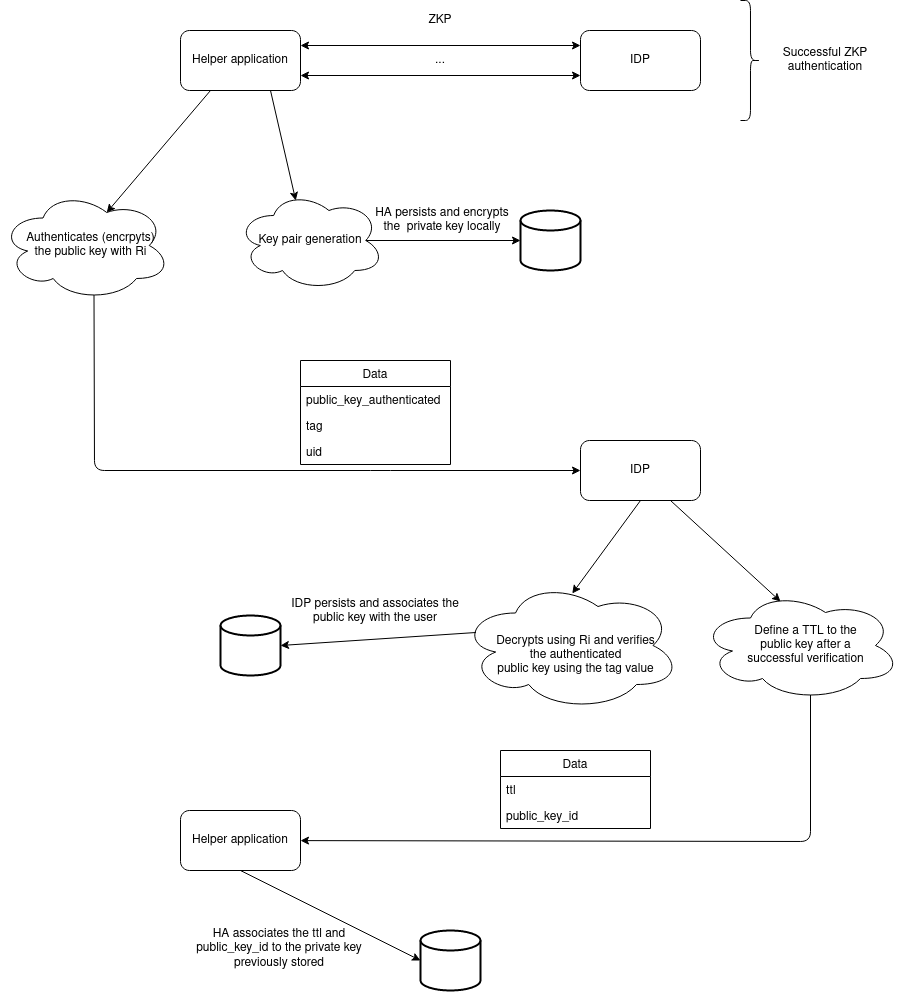
\includegraphics[width=\textwidth]{img/pub_key_upload.png}
    \centering
\end{figure}

\begin{enumerate}
    \item Após o processo de autenticação com ZKP, a \textit{helper application} gera uma par de chaves assimétricas RSA, onde armazena de forma cifrada a chave privada (usando como segredo uma derivação da  chave mestra - \ref{chaveiro} e a senha da conta associada ao processo de autenticação atual) e faz a cifra da chave publica usando o algoritmo AES cujo segredo usado é $R_i$ (ultima resposta calculada durante o protocolo ZKP). Por fim, a aplicação envia o uid para identificar a instância do protocolo de autenticação, o conteúdo cifrado e autenticado da chave publica e o valor de tag que representa o MAC \cite{mac} gerado pelo AES devido ao modo utilizado (SIV).
    \item O idp após receber o pedido de \textit{upload} da chave assimétrica, verifica se o conteúdo da chave publica recebida está corretamente autenticado (isto é, confirmação que foi enviado pela \textit{helper application} e que não foi adulterado no canal de comunicação) verificado o valor da \textit{tag}, caso exista uma verificação positiva o servidor decifra usando $R_i$ e armazena localmente a chave publica.  Após este processo de verificação e armazenamento o idp define o TTL (Time to live), um ano, desta chaves assimétricas e mapeia este valor com a chave recebida. Finalmente, este envia para a \textit{helper application} o id associado ao armazenamento da chave publica e o ttl definido.
    \item Finalizando, a \textit{helper application} necessita de armazenar os valores do ttl e \textit{public\_key\_id}.
\end{enumerate}

\quad Uma vez que para realizar o processo de autenticação usando credenciais assimétricas é necessário fazer a partilha da chave publica com o IDP, este \textit{upload} da chave deve ser autenticado e portanto, neste caso isto é implementado usando um segredo partilhado entre as duas entidades, que neste caso é a ultima resposta calculada durante o protocolo de autenticação. A autenticação é realizada cifrando o conteúdo da chave publica com o algoritmo criptográfico AES cujo segredo é $R_i$ que gera, também, um valor de MAC (tag), deste modo aquando da receção da chave publica pelo IDP este consegue verificar que a mensagem foi efetivamente enviada pela \textit{helper application} e que o conteúdo cifrado não foi alterado uma vez que o segredo usado no processo de cifra é uma resposta calculada (que nunca circulou no canal de comunicação) no protocolo anterior (ZKP).


\quad Agora, o processo de autenticação usando estas credenciais assimétricas vai ser explicado e detalhado para tentar esclarecer quaisquer duvidas que surjam.


\begin{figure}[H]
    \caption{Autenticação usando as credenciais assimétricas}
    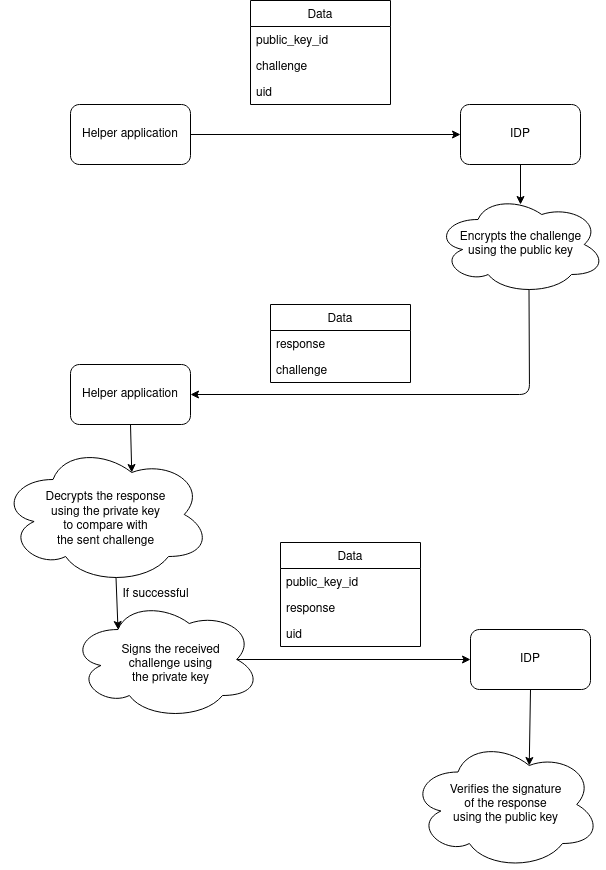
\includegraphics[width=\textwidth]{img/pub_key_auth.png}
    \centering
\end{figure}

\begin{enumerate}
    \item De forma semelhante, ao protocolo de conhecimento nulo a \textit{helper application} inicializa este método de autenticação ao enviar um desafio gerado aleatoriamente, o id da chave publica e o uid.
    \item O idp após receber os dados, cifra o desafio recebido com a chave publica identificada pelo \textit{public\_key\_id} e gera também um desafio que depois são ambos enviados para a \textit{helper application}.
    \item Após receção dos dados, a \textit{helper application} decifra a resposta recebida e compara o valor decifrado com o desafio enviado anteriormente, caso estes valores sejam iguais significa que a chave publica usada pelo \textit{idp} é a chave correta associada à chave privada. Para que o \textit{idp} possa verificar a legitimidade da \textit{helper application} esta assina o desafio recebido com a chave privada e envia este valor juntamente, com o id da chave publica e o uid.
    \item Por fim, o IDP verifica a assinatura realizada com a chave publica e caso esta assinatura seja válida o processo de autenticação é terminado com sucesso.
\end{enumerate}

\quad É importante referir que caso alguma das verificações falhe o protocolo é interrompido e se no momento do uso das chaves para as operações necessárias neste protocolo estiverem inválidas em termos temporais, o protocolo é interrompido e as credencias assimétricas são eliminadas de ambas as entidades, ou seja, antes de realizar qualquer processo criptográfico com as chaves assimétricas as respetivas entidades devem verificar se o ttl do par de credenciais é valido. Por fim, para aumentar a robustez desta implementação e pelo facto deste método de autenticação ser um processo complementar ou secundário, caso exista alguma falha neste protocolo, as entidades realizam a autenticação usando o protocolo de conhecimento nulo.

\quad Apesar de no enunciado do projeto sugerir realizar um protocolo de desafio-resposta para verificar que o \textit{upload} da chave publica foi executado corretamente, neste caso devido ao modo de operação do AES já existe esta validação devido ao valor de MAC, isto é, se o IDP conseguiu decifrar o conteúdo enviado pela \textit{helper application} significa que todo o processo ocorreu como esperado e que o processo de autenticação usando estas chaves assimétricas pode ser executado.


\subsection{Performance dos protocolos de autenticação}

\quad Numa fase experimental é sempre interessante perceber as diferenças temporais entre os dois tipos de protocolo de autenticação. Portanto para calcular os tempos de execução, foram contabilizados 10 execuções de cada protocolo para no final ser calculada a média dos tempos.

\begin{itemize}
    \item \textbf{ZKP} com N = 200: 2.727698564529419
    \item \textbf{Credenciais Assimétricas}: 0.8922686576843262
\end{itemize}


\quad Como é observável existe uma diferença considerável entre os tempos de execução dos dois protocolos, cerca de 2 segundos, é óbvio que aos "olhos" do utilizador esta diferença não parece problemática, contudo, no ambiente do servidor ter um protocolo que demora cerca de dois segundos (pode demorar mais se o numero de iterações for maior) a executar pode dificultar a gestão de recursos computacionais uma vez que o IDP tem que estar apto para receber múltiplas conexões simultaneamente.